\documentclass{article}
\usepackage{graphicx}
\usepackage{amsmath}
\usepackage{booktabs}
\usepackage{siunitx}
\usepackage{float}

\title{Homework 2 - EE4520 Analog CMOS Design 1}
\author{Daniel Tyukov \\ Student Number: 5714699 \\ Electrical Engineering, TU Delft}
\date{February 2026}

\begin{document}

\maketitle

\tableofcontents

\clearpage

\section{Deliverable 1 - Table of Results}
\begin{table}[H]
\centering
\small
\sisetup{detect-weight=true,detect-family=true}
\begin{tabular}{@{}c l l l l@{}}
\toprule
\# & Design Item & Unit & Spec & Achieved \\
\midrule
1  & Design Number & [-] & 27 & 27 \\
2  & SNR & [dB] & 80.64 & 80.85 \\
3  & $A_{\text{settle}}$ & [dB] & 63 & 63.32 \\
4  & $T_{\text{settle}}$ & [ns] & 2800 & 2800 \\
5  & $BW_{cl}$ from open-loop AC sims & [MHz] & --- & 0.329 \\
6  & $BW_{cl}$ from closed-loop AC sims & [MHz] & --- & 0.329 \\
7  & Time-constant $\tau_{cl}$ from closed-loop AC sims & [ns] & --- & 483.1 \\
8  & $T_{40\text{dB}}$ (time to reach accuracy of 40 dB) & [ns] & --- & 1396.9 \\
9  & $T_{48.69\text{dB}}$ (time to reach accuracy of 48.69 dB) & [ns] & --- & 1894.3 \\
10 & Time-constant $\tau_{cl}$ from transient sim & [ns] & --- & 497.4 \\
11 & Power dissipation & [mW] & Lowest possible & 0.1119 \\
12 & $I(V_{dd})$ & [mA] & Lowest possible & 0.0622 \\
13 & Total integrated noise & [\si{\micro\volt}] & --- & 76.93 \\
14 & Input step voltage & [mV] & 150 & 150 \\
15 & Output step voltage & [V] & 1.2 & 1.2 \\
16 & $C_{in}$ & [pF] & --- & 18 \\
17 & $C_{fb}$ & [pF] & --- & 2.25 \\
18 & $C_{load}$ & [pF] & --- & 18 \\
19 & $C_{CM}$ & [pF] & --- & 2.25 \\
20 & $R_{big}$ & [G$\Omega$] & Big & 100 \\
21 & $C_{big}$ & [nF] & Big & 1000 \\
22 & Bonus points on FoM$_{dB}$ & [-] & 0 & 0 \\
23 & FoM$_{lin}=2\pi\cdot$Power$\cdot T_{8.6\text{dB}}$/SNR$_{lin}^2$ & [J] & $\le 3.98\mathrm{e}{-18}$ & $3.02\mathrm{e}{-18}$ \\
24 & FoM$_{dB}=-10\log_{10}(\mathrm{FoM}_{lin})$ & [dB] & $\ge 174.00$ & 175.20 \\
\bottomrule
\end{tabular}
\end{table}

\subsection*{Computation notes}
\begin{itemize}
\item $BW_{cl}$ (open-loop): frequency where $|A\beta|=1$ $\Rightarrow$ $0.329~\mathrm{MHz}$.
\item $BW_{cl}$ (closed-loop): $-3~\mathrm{dB}$ frequency of closed-loop gain $\Rightarrow$ $0.329~\mathrm{MHz}$.
\item $\tau_{cl}$ (AC): $\tau_{cl}=\dfrac{1}{2\pi BW_{cl}}=\dfrac{1}{2\pi\cdot 329\mathrm{kHz}}=483.1~\mathrm{ns}$.
\item $\tau_{cl}$ (transient): $\tau_{cl}=T_{48.69\text{dB}}-T_{40\text{dB}}=1894.3-1396.9=497.4~\mathrm{ns}$.
\item SNR: $\mathrm{SNR}_{dB}=20\log_{10}\!\left(\dfrac{0.8485}{76.93\cdot 10^{-6}}\right)=80.85~\mathrm{dB}$.
\item Power: $P=\overline{I(V_{dd})}\cdot 1.8~\mathrm{V}=62.2~\mu\mathrm{A}\cdot 1.8~\mathrm{V}=0.1119~\mathrm{mW}$.
\end{itemize}

\subsection*{Design parameters}
ScaleA $=0.25$, Mn34 $=200$, $C_{in}=18~\mathrm{pF}$, $I_{bm}=350~\mu\mathrm{A}$, $W=1~\mu\mathrm{m}$, $L=0.18~\mu\mathrm{m}$, Mp $=60$, Mn $=11$, mp\_ratio $=5.45$, Rn $=5.8$, Rp $=7.5$, Aadd $=100$.

\clearpage

\section{Deliverable 2 - Schematic with All Node Voltages}
\begin{figure}[H]
\centering
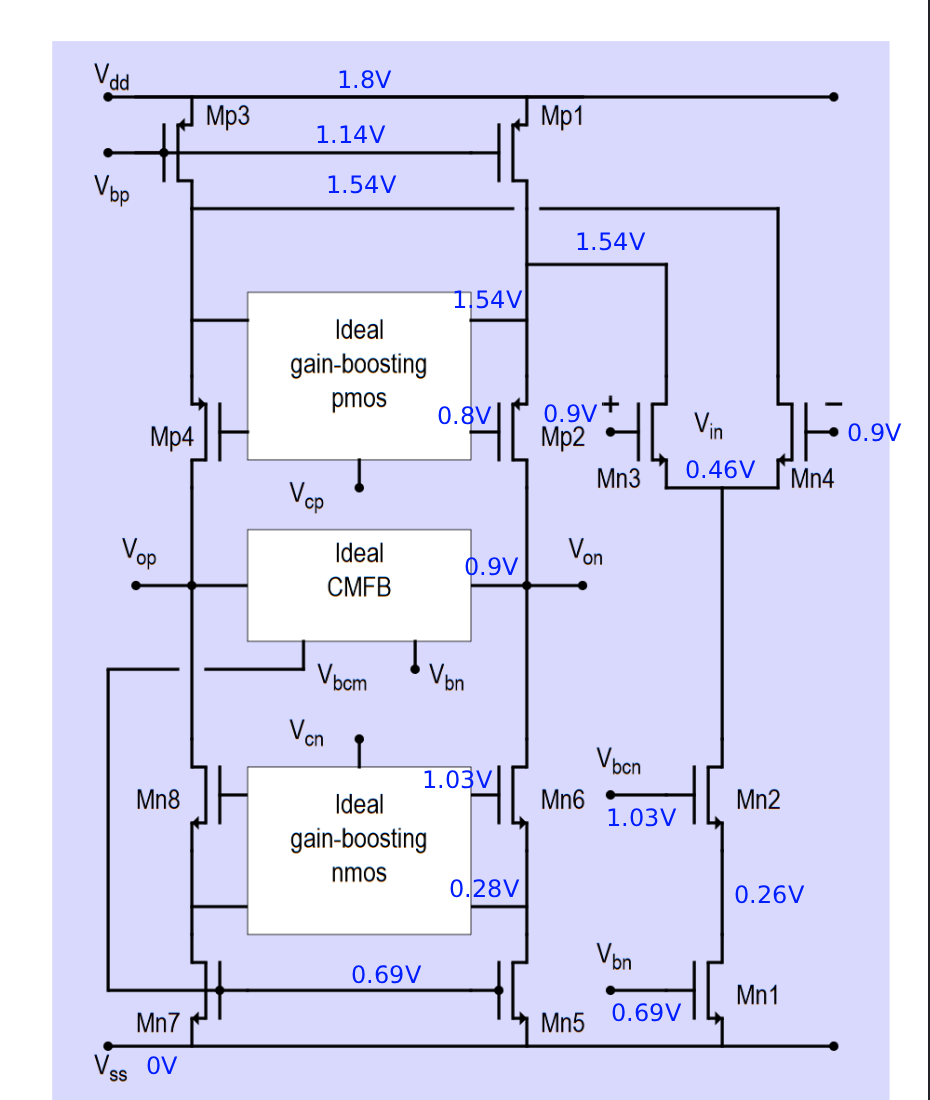
\includegraphics[width=\textwidth]{deliverable_2_with_all_node_voltages.png}
\caption{Folded-cascode OpAmp with ideal gain-boosting and annotated DC node voltages.}
\end{figure}

\clearpage

\section{Deliverable 3 - Schematic with All Branch Currents}
\begin{figure}[H]
\centering
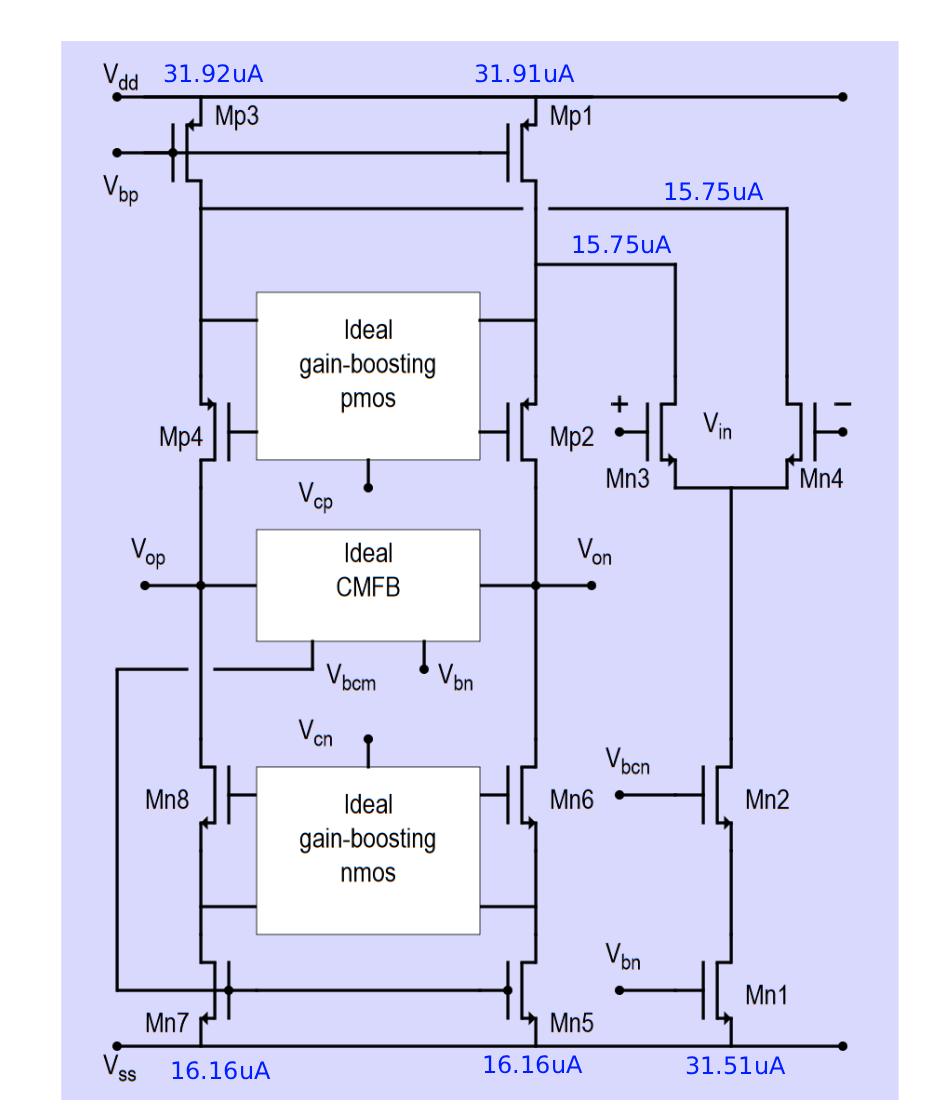
\includegraphics[width=\textwidth]{deliverable_3_with_all_branch_currents.png}
\caption{Folded-cascode OpAmp with annotated DC branch currents.}
\end{figure}

\clearpage

\section{Deliverable 4 - Bode Diagram of $A$ and $A\beta$ (Gain and Phase)}
\subsection{Unloaded open-loop simulation}
\begin{figure}[H]
\centering
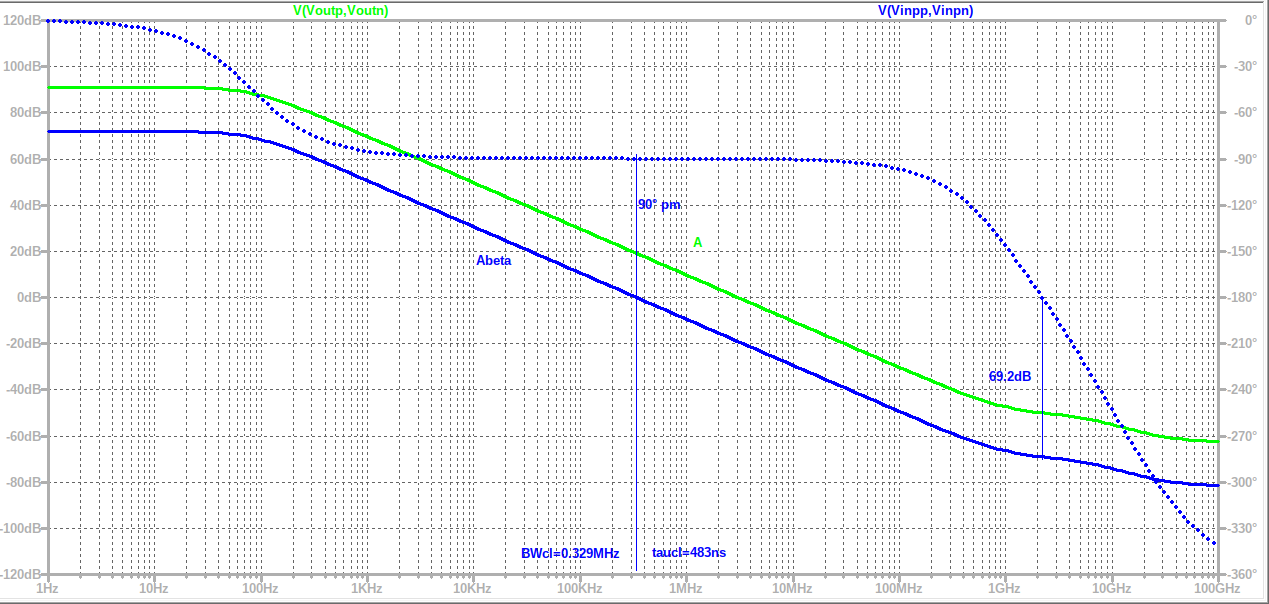
\includegraphics[width=\textwidth]{deliverable_4_plot_bode-diagram-A-Abeta-with-gain-and-phase-unloaded.png}
\caption{Bode diagram of open-loop gain $A$ and loop gain $A\beta$ (unloaded).}
\end{figure}

Key extracted metrics:
\begin{itemize}
\item Closed-loop bandwidth from unity loop-gain crossing: $BW_{cl}=0.329~\mathrm{MHz}$.
\item Closed-loop time-constant: $\tau_{cl}=\dfrac{1}{2\pi BW_{cl}}=483.1~\mathrm{ns}$.
\item Low-frequency separation between $A$ and $A\beta$ equals $20\log_{10}(8)=18.06~\mathrm{dB}$, consistent with $A_{cl}=8$.
\end{itemize}

\subsection{Loaded open-loop simulation (with replica loading)}
\begin{figure}[H]
\centering
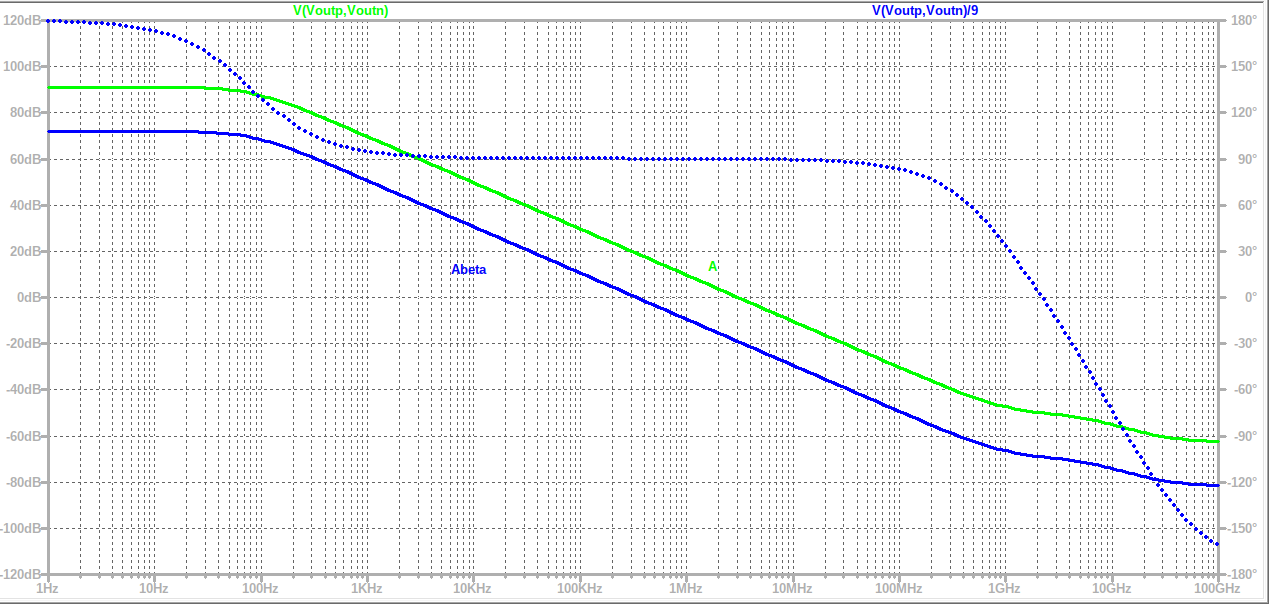
\includegraphics[width=\textwidth]{deliverable_4_plot_bode-diagram-A-Abeta-with-gain-and-phase-loaded.png}
\caption{Bode diagram of open-loop gain $A$ and loop gain $A\beta$ (loaded).}
\end{figure}

The loaded and unloaded cases yield essentially the same $BW_{cl}$ and stable behavior (high phase margin), indicating limited sensitivity to the applied replica loading for this configuration.

\clearpage

\section{Deliverable 5 - Bode Diagram of Closed-Loop Gain (Gain and Phase)}
\begin{figure}[H]
\centering
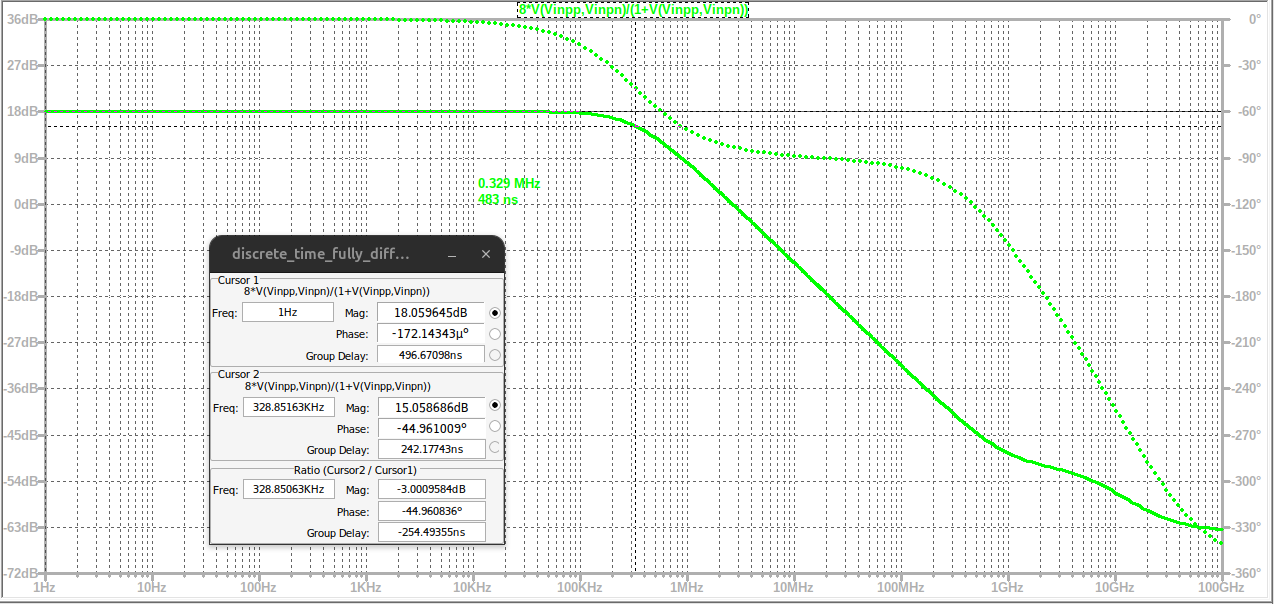
\includegraphics[width=\textwidth]{deliverable_5_plot_bode-diagram-closed-loop-gain-with-gain-and-phase.png}
\caption{Closed-loop transfer function magnitude and phase.}
\end{figure}

From the plot:
\begin{itemize}
\item Passband gain: $20\log_{10}(8)=18.06~\mathrm{dB}$.
\item $-3~\mathrm{dB}$ bandwidth: $BW_{cl}\approx 0.329~\mathrm{MHz}$.
\item Corresponding time constant: $\tau_{cl}=\dfrac{1}{2\pi BW_{cl}}=483.1~\mathrm{ns}$.
\end{itemize}

The $BW_{cl}$ obtained here matches the unity-crossing of $|A\beta|$ from Deliverable 4, as expected for a predominantly first-order closed-loop system.

\clearpage

\section{Deliverable 6 - Settling Accuracy Versus Time}
The settling accuracy is evaluated using:
\[
\mathrm{Accuracy}_{dB}(t)=20\log_{10}\!\left(\frac{1.2}{|V(\mathrm{virtualground})|+1\mathrm{n}}\right).
\]

\begin{figure}[H]
\centering
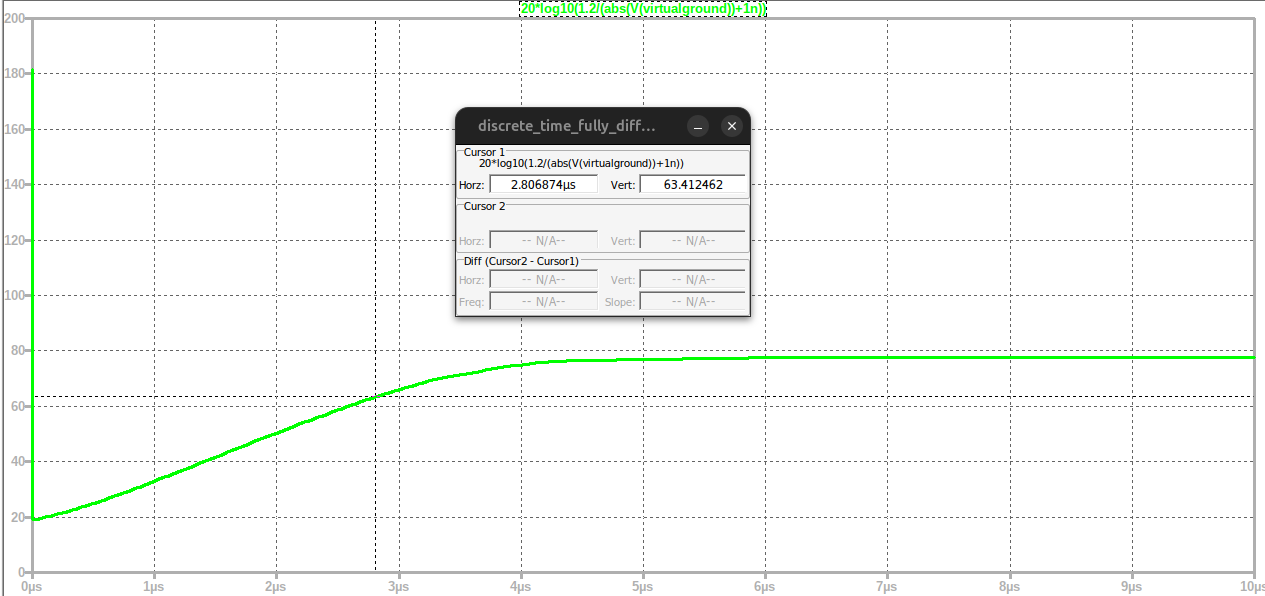
\includegraphics[width=\textwidth]{deliverable_6_plot_settling-accuracy-vs-time.png}
\caption{Settling accuracy versus time.}
\end{figure}

At $T_{\text{settle}}=2.8~\mu\mathrm{s}$, the achieved accuracy is $\approx 63.3~\mathrm{dB}$, meeting the $63~\mathrm{dB}$ target.

\clearpage

\section{Deliverable 7 - Settling Accuracy with $T_{\text{settle}}$, $T_{40\text{dB}}$, and $T_{48.69\text{dB}}$}
\begin{figure}[H]
\centering
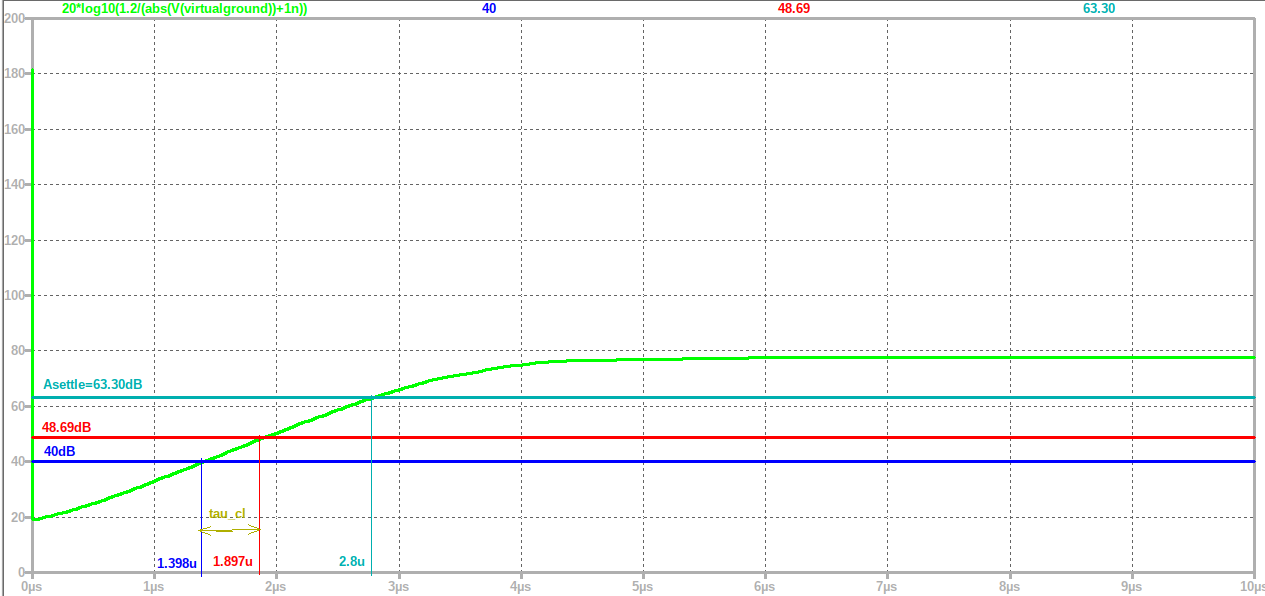
\includegraphics[width=\textwidth]{deliverable_7_plot_settling-accuracy-vs-time-estimated-time-const.png}
\caption{Settling accuracy with timing markers for time-constant estimation.}
\end{figure}

Extracted timing points:
\begin{itemize}
\item $T_{40\text{dB}}=1396.9~\mathrm{ns}$,
\item $T_{48.69\text{dB}}=1894.3~\mathrm{ns}$,
\item $\tau_{cl}=T_{48.69\text{dB}}-T_{40\text{dB}}=497.4~\mathrm{ns}$.
\end{itemize}

Comparison of $\tau_{cl}$:
\begin{table}[H]
\centering
\begin{tabular}{@{}l c@{}}
\toprule
Source & $\tau_{cl}$ [ns] \\
\midrule
From AC ($BW_{cl}=0.329~\mathrm{MHz}$) & 483.1 \\
From transient ($T_{48.69\text{dB}}-T_{40\text{dB}}$) & 497.4 \\
\bottomrule
\end{tabular}
\end{table}

\clearpage

\section{Deliverable 8 - Output Noise Power Density Versus Frequency}
\begin{figure}[H]
\centering
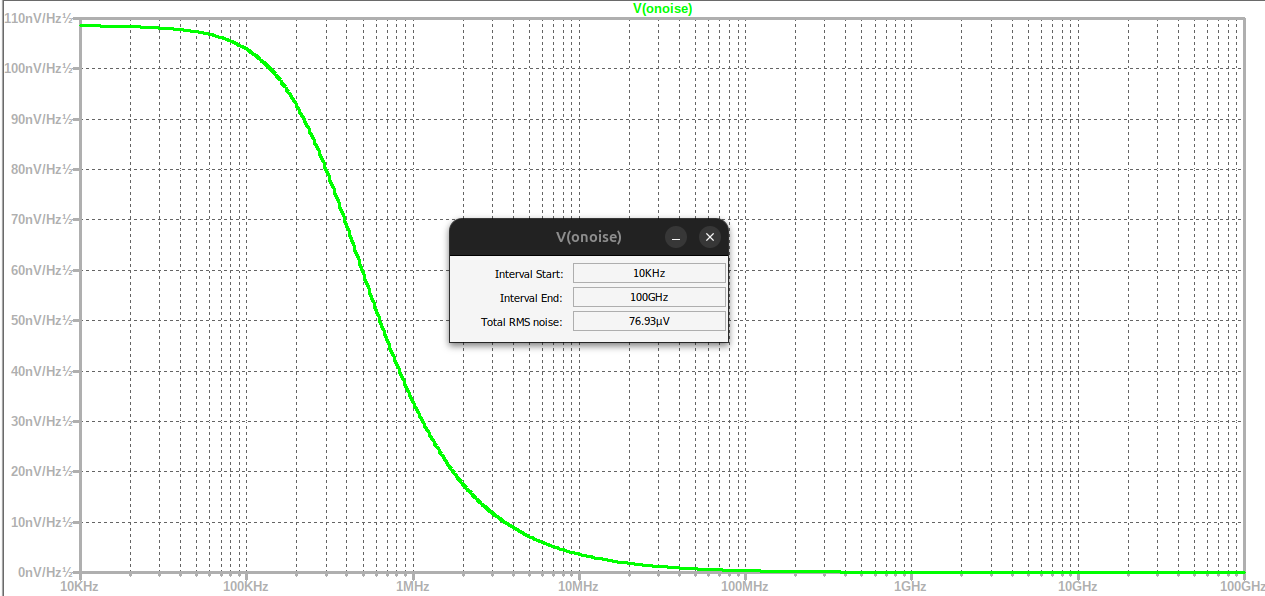
\includegraphics[width=\textwidth]{deliverable_8_plot_output-noise-power-density-vs-freq.png}
\caption{Output noise density versus frequency and integrated RMS noise (10 kHz -- 100 GHz).}
\end{figure}

Integrated output RMS noise (10 kHz to 100 GHz): $76.93~\mu\mathrm{V}_{rms}$, yielding:
\[
\mathrm{SNR}_{dB}=20\log_{10}\!\left(\frac{0.8485}{76.93\cdot 10^{-6}}\right)=80.85~\mathrm{dB}.
\]

\clearpage

\section{Deliverable 9 - Design Process Description}

\subsection{Design constraints and dominant trade-offs}
This design is primarily noise-limited: the SNR requirement of $80.64~\mathrm{dB}$ constrains the integrated output noise to
$\le 78.8~\mu\mathrm{V}_{rms}$, while the settling target ($T_{\text{settle}}=2.8~\mu\mathrm{s}$) sets the required closed-loop bandwidth. Key observations:

\vspace{-2mm}
\begin{itemize}
\setlength{\itemsep}{2pt}
\item Increasing capacitor values reduces integrated noise (via $kT/C$) but increases required charge transfer, thus requiring higher $g_m$ (more current) to maintain settling.
\item The input pair (MN3/MN4) dominates thermal noise; biasing it in weak/moderate inversion maximizes $g_m/I_D$ and improves noise efficiency.
\item Current-source devices (MN1, MN5--8, MP1--4) contribute noise; biasing them closer to strong inversion reduces their relative contribution while maintaining headroom.
\item Global scaling (ScaleA) increases all currents, improving speed/noise but increasing power roughly proportionally.
\item Therefore, $C_{in}$ and input-pair sizing are the main levers to meet SNR at minimum power.
\end{itemize}

\vspace{-2mm}

\subsection{Design steps}
\begin{enumerate}
\setlength{\itemsep}{2pt}
\item \textbf{Capacitor selection:} Choose $C_{in}=18~\mathrm{pF}$ with $C_{fb}=C_{in}/8=2.25~\mathrm{pF}$, $C_{load}=C_{in}$, and $C_{CM}=C_{fb}$ to achieve $76.93~\mu\mathrm{V}_{rms}$ noise.
\item \textbf{Input pair sizing:} Use large multiplicity ($\mathrm{Mn34}=200$) to increase effective $g_m$ at low current and reduce dominant noise.
\item \textbf{Power minimization:} Set $\mathrm{ScaleA}=0.25$ and $I_{bm}=350~\mu\mathrm{A}$, yielding $\overline{I(V_{dd})}\approx 62.2~\mu\mathrm{A}$ and $P\approx 0.1119~\mathrm{mW}$. Sweeps of $I_{bm}$ and $C_{in}$ identify the minimum-power solution.
\end{enumerate}

\vspace{-2mm}

\subsection{Link between open-loop, closed-loop, and settling results}
The unity crossing of $|A\beta|$ gives:
\[
BW_{cl}\approx 0.329~\mathrm{MHz}, \quad
\tau_{cl,\mathrm{AC}}=\frac{1}{2\pi BW_{cl}}=483.1~\mathrm{ns}.
\]
The separation $20\log_{10}(8)\approx 18.06~\mathrm{dB}$ confirms $A_{cl}=8$, and the closed-loop AC simulation gives the same $BW_{cl}$.

From transient:
\[
\tau_{cl,\mathrm{tran}}=T_{48.69\text{dB}}-T_{40\text{dB}}=497.4~\mathrm{ns},
\]
which is $\approx3\%$ higher than $\tau_{cl,\mathrm{AC}}$. At $2.8~\mu\mathrm{s}$,
$A_{\text{settle}}\approx 63.3~\mathrm{dB}$, $\mathrm{SNR}=80.85~\mathrm{dB}$, and $\mathrm{FoM_{dB}}=175.20~\mathrm{dB}$.


\clearpage
\appendix

\section{Appendix - Simulation Schematics}

\subsection{Reference Schematic with Voltages and Currents}
\begin{figure}[H]
\centering
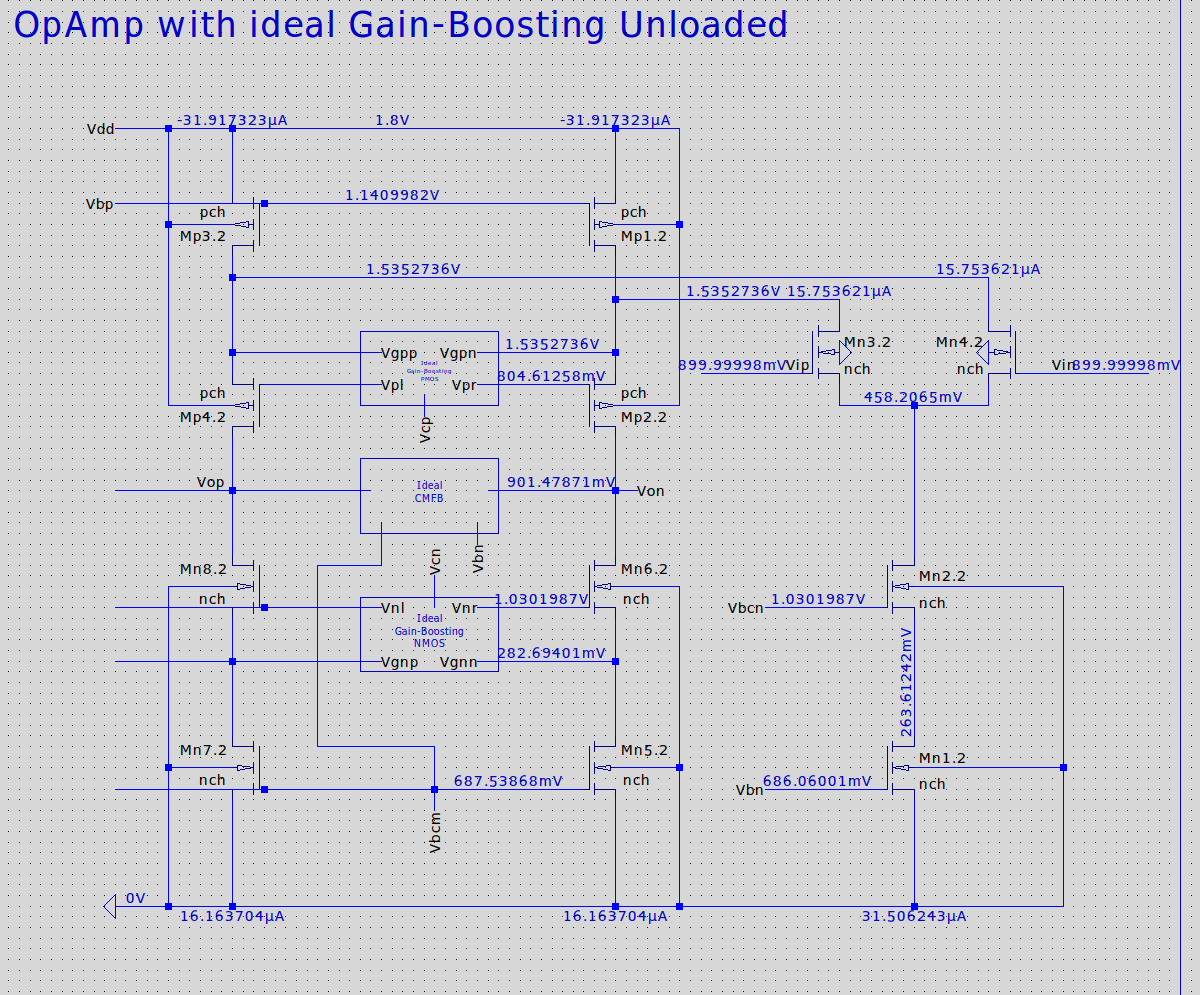
\includegraphics[width=\textwidth]{appendix_schematic_voltages_currents_ref.png}
\caption{Complete OpAmp schematic with annotated node voltages and branch currents.}
\end{figure}

\clearpage

\subsection{Open-Loop AC Simulation (Unloaded)}
\begin{figure}[H]
\centering
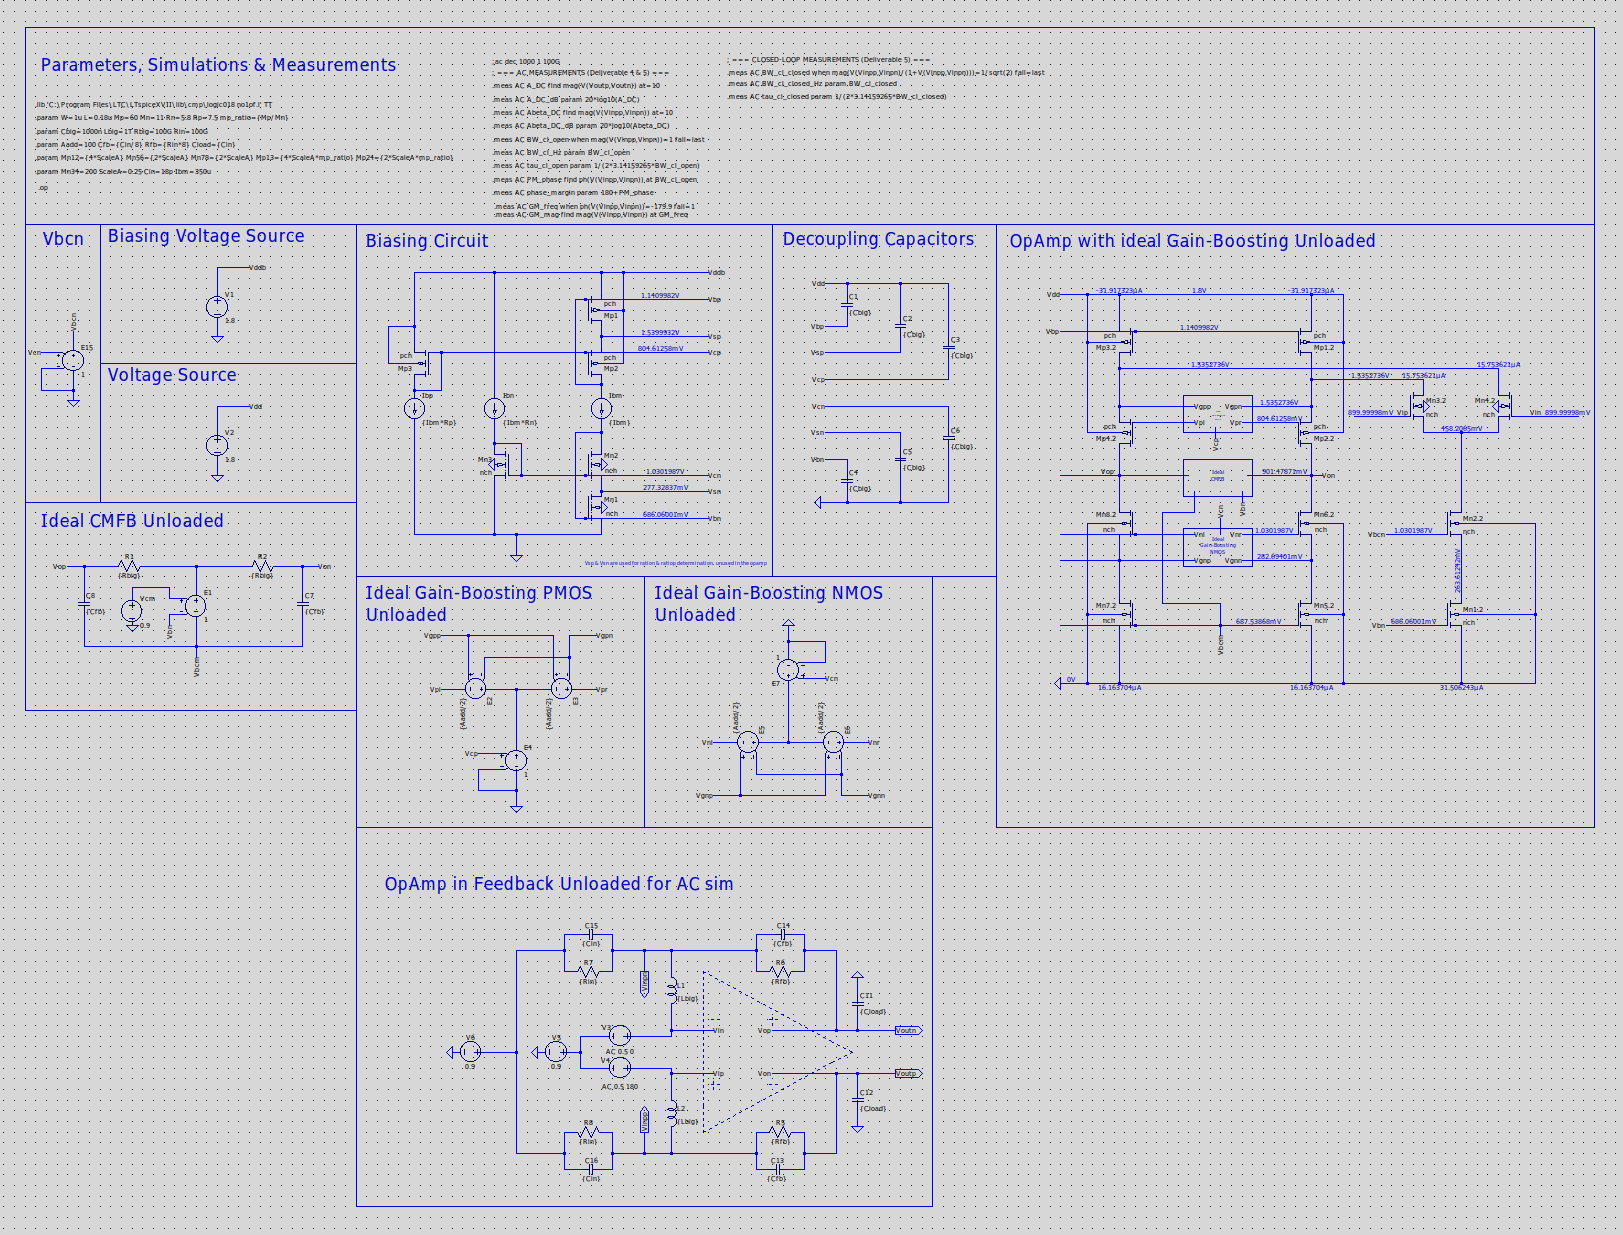
\includegraphics[width=\textwidth]{appendix_schematic_unloaded_ac.png}
\caption{Schematic used for open-loop AC simulation without replica loading.}
\end{figure}

\clearpage

\subsection{Open-Loop AC Simulation (Loaded)}
\begin{figure}[H]
\centering
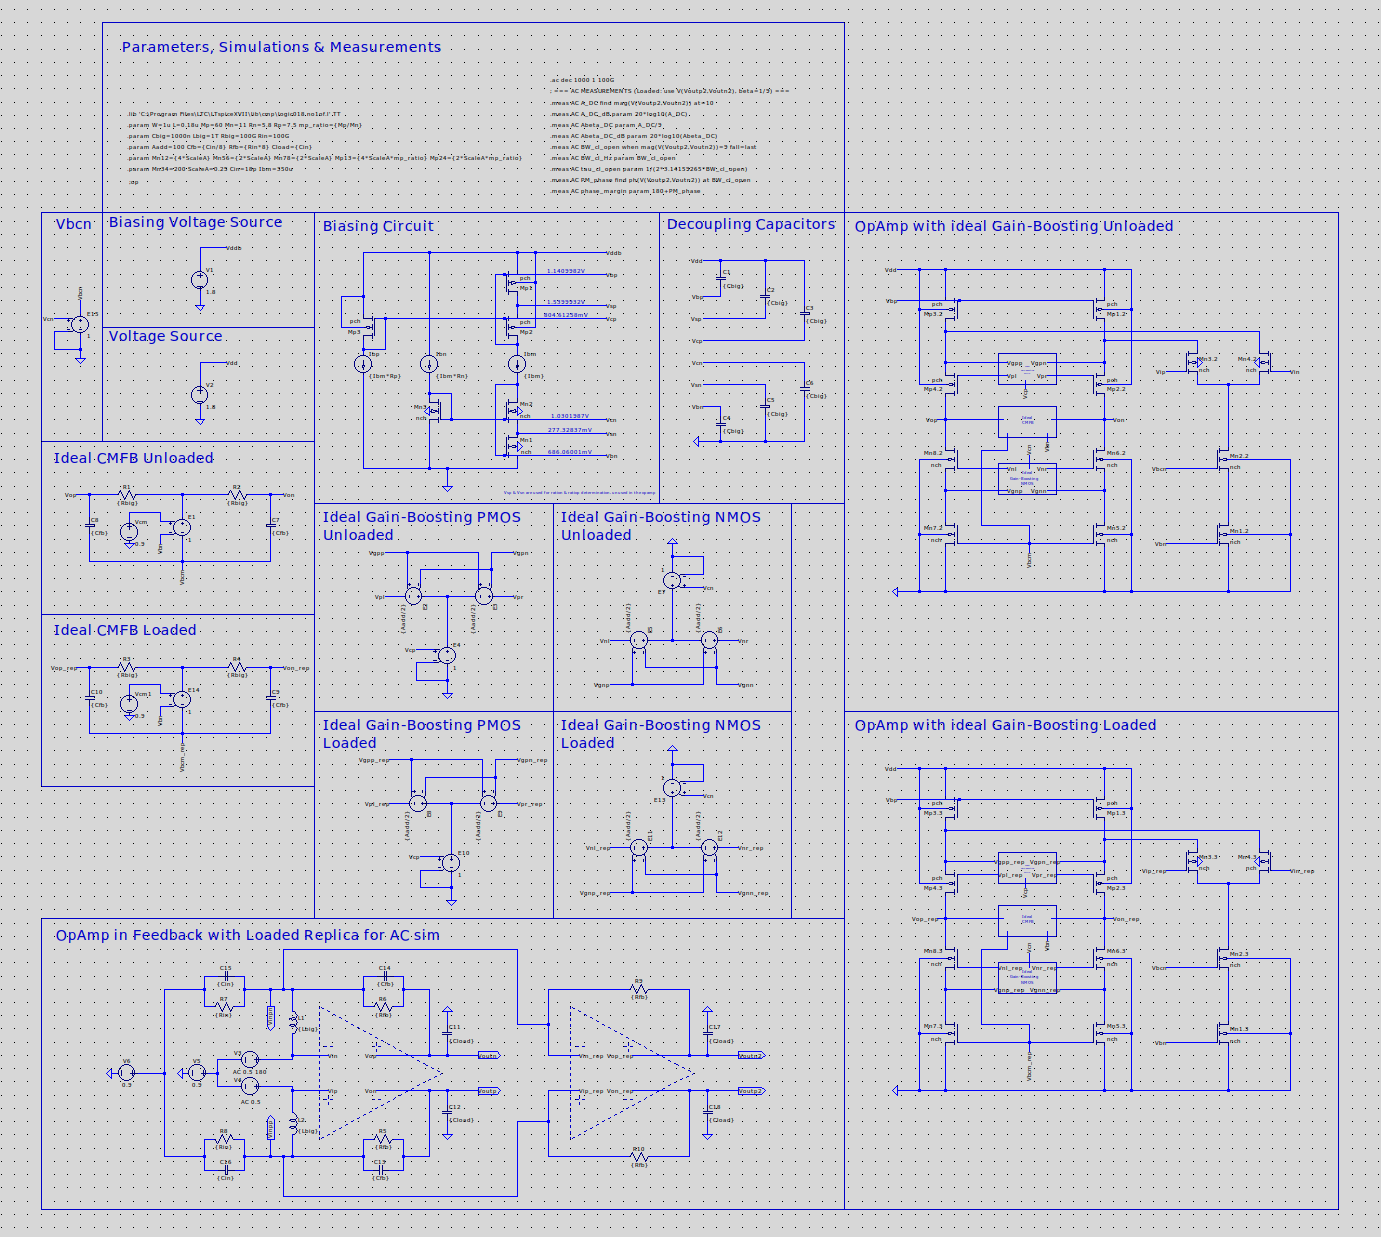
\includegraphics[width=\textwidth]{appendix_schematic_loaded_ac.png}
\caption{Schematic used for open-loop AC simulation with replica loading.}
\end{figure}

\clearpage

\subsection{Closed-Loop Noise Simulation}
\begin{figure}[H]
\centering
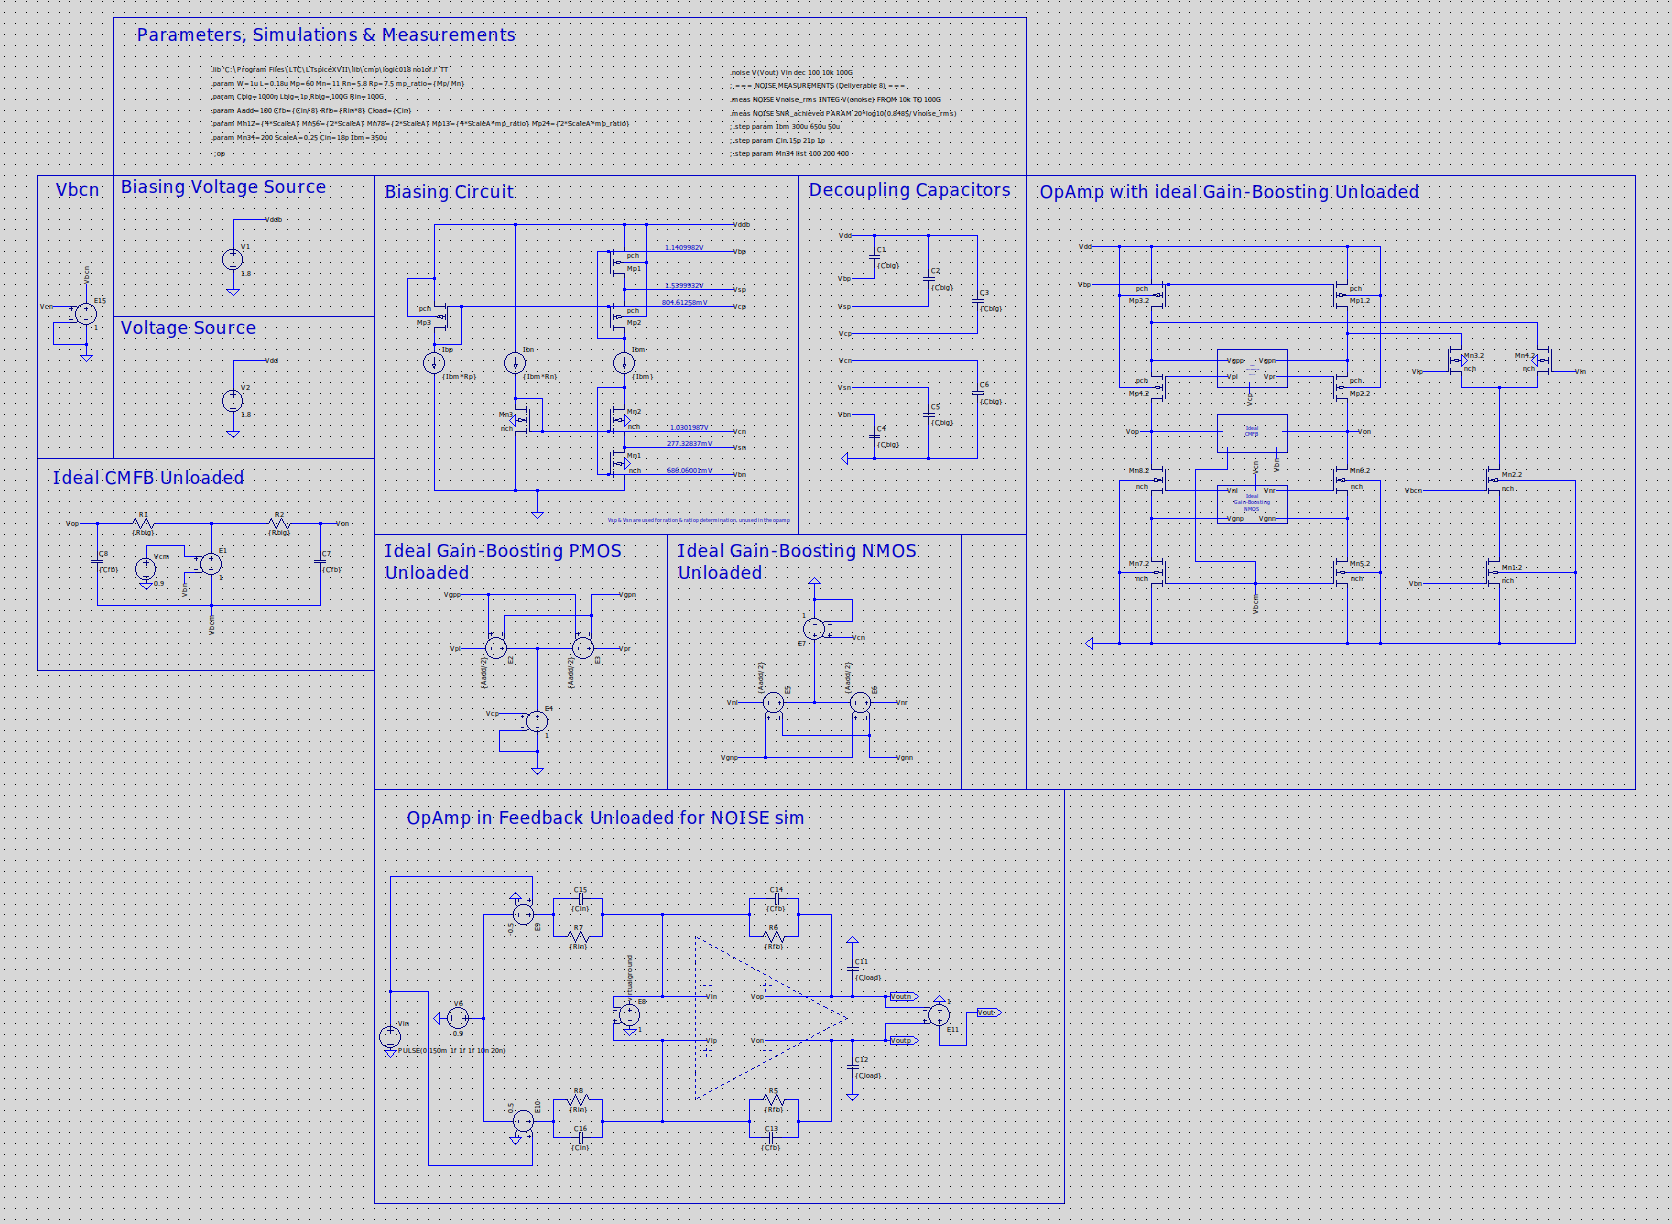
\includegraphics[width=\textwidth]{appendix_schematic_unloaded_noise.png}
\caption{Schematic used for output noise simulation in closed-loop configuration.}
\end{figure}

\clearpage

\subsection{Closed-Loop Transient Simulation}
\begin{figure}[H]
\centering
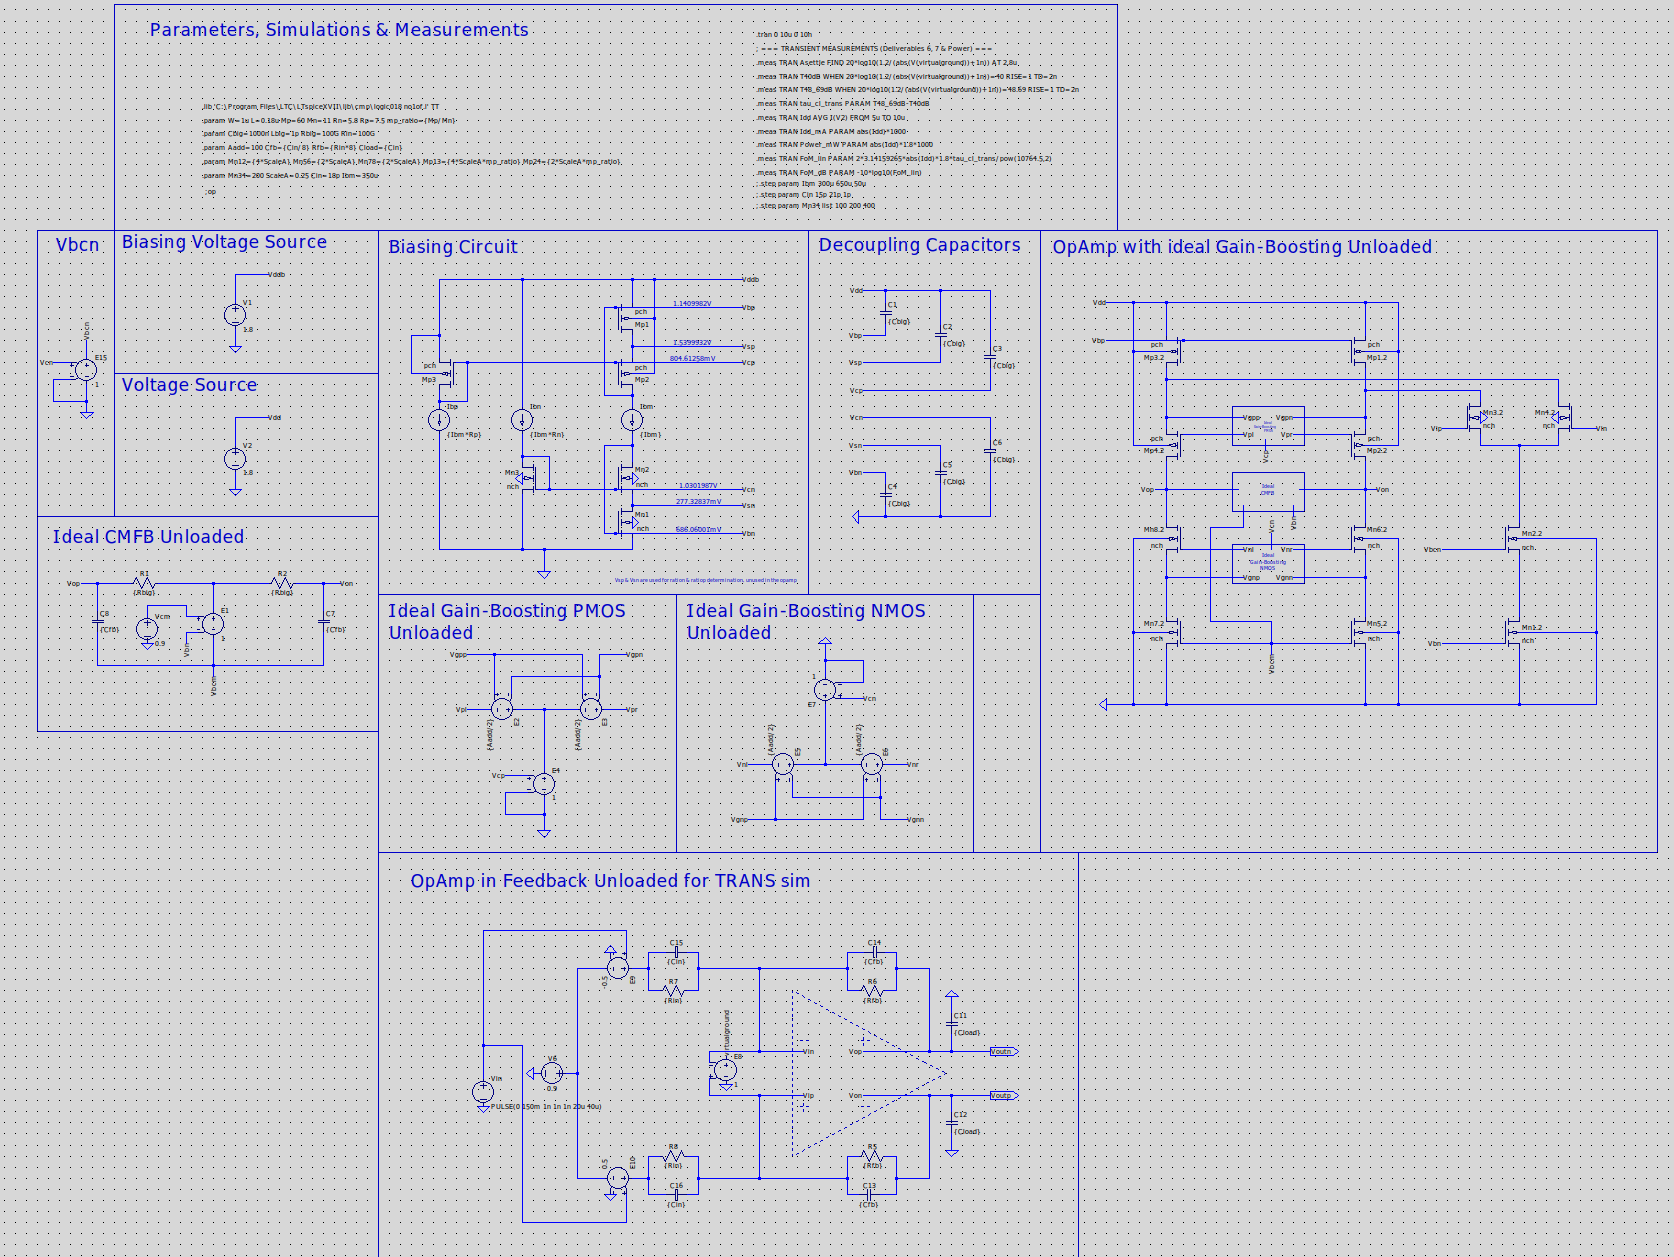
\includegraphics[width=\textwidth]{appendix_schematic_unloaded_trans.png}
\caption{Schematic used for transient settling simulations.}
\end{figure}


\end{document}
